\section{Cálculo diferencial}

El cálculo diferencial estudia cómo cambian las funciones. Sus herramientas principales son las derivadas, que permiten analizar la variación instantánea de una magnitud.

\subsection{Derivadas}

La derivada de una función mide la tasa de cambio instantánea. Se define como:

\begin{figure}[H]
    \centering
    \captionsetup{width=0.5\textwidth}
    \caption{Interpretación gráfica de la derivada}
    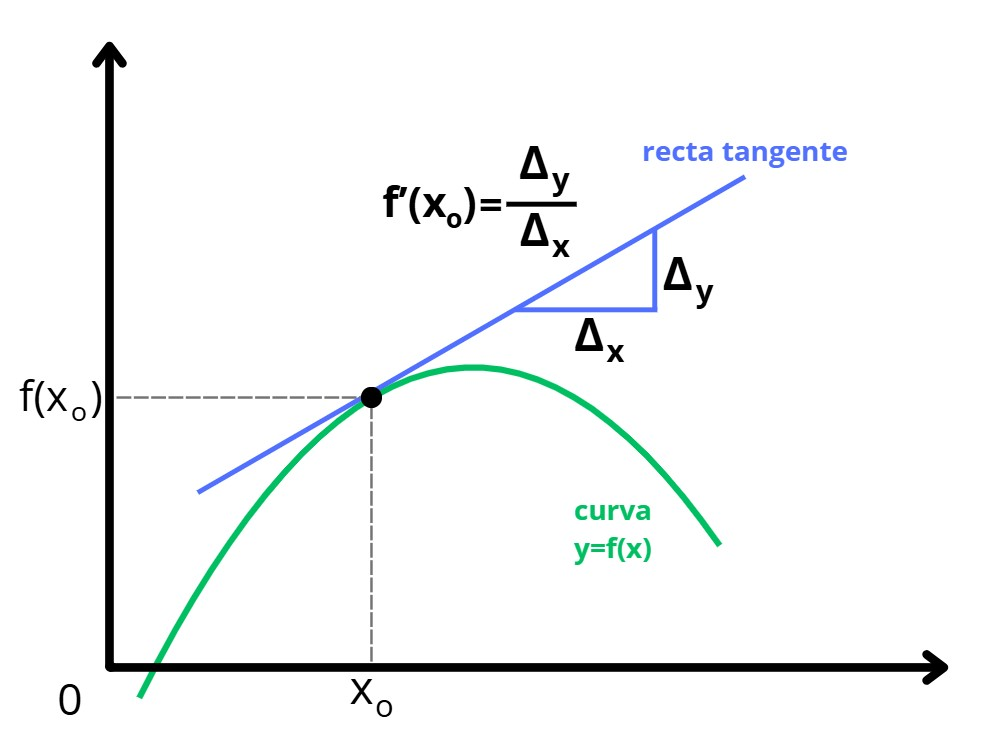
\includegraphics[width=0.6\textwidth]{images/cinematicGraphics/derivative.jpg}
    \caption*{Nota: La derivada se interpreta como la pendiente de la recta tangente a la curva en un punto.}
\end{figure}

\vspace{-40pt}

\[
f'(x) = \lim_{\Delta x \to 0} \frac{f(x+\Delta x) - f(x)}{\Delta x}
\]

\subsubsection{Interpretación}

Geométricamente, la derivada representa la pendiente de la recta tangente a la curva en un punto.

Físicamente, por ejemplo:
\[
v = \frac{dx}{dt}
\]
representa la velocidad como cambio de posición respecto al tiempo.

\subsubsection{Reglas de derivación}

Las reglas de derivación permiten calcular derivadas de manera rápida sin usar directamente la definición.

\begin{itemize}

\item \textbf{Regla de la suma:}

\[
\frac{d}{dx}[f(x) + g(x)] = \frac{df}{dx} + \frac{dg}{dx}
\]

\textbf{Ejemplo:}
\[
\frac{d}{dx}(x^2 + x) = \frac{d}{dx}(x^2) + \frac{d}{dx}(x) = 2x + 1
\]

\item \textbf{Regla del producto:}

\[
\frac{d}{dx}[f(x)g(x)] = f'(x)g(x) + f(x)g'(x)
\]

\textbf{Ejemplo:}
\[
\frac{d}{dx}(x^2 \cdot x) = \frac{d}{dx}(x^2)\cdot x + x^2 \cdot \frac{d}{dx}(x)
\]
\[
= 2x \cdot x + x^2 \cdot 1 = 2x^2 + x^2 = 3x^2
\]

\item \textbf{Regla del cociente:}

% chktex-file 3
\[
\frac{d}{dx}\left[\frac{f(x)}{g(x)}\right] = \frac{f'(x)g(x) - f(x)g'(x)}{g(x)^2}
\]

\textbf{Ejemplo:}
\[
\frac{d}{dx}\left(\frac{x^2}{x}\right)
= \frac{\frac{d}{dx}(x^2)\cdot x - x^2 \cdot \frac{d}{dx}(x)}{x^2}
\]
\[
= \frac{2x \cdot x - x^2 \cdot 1}{x^2}
= \frac{2x^2 - x^2}{x^2} = 1
\]

\item \textbf{Regla de la cadena:}

\[
\frac{d}{dx}f(g(x)) = f'(g(x)) \cdot g'(x)
\]

\textbf{Ejemplo:}
\[
\frac{d}{dx}(x^2 + 1)^2 = \frac{d}{dx}\left[(x^2 + 1)^2\right]
\]
\[
= 2(x^2 + 1)\cdot \frac{d}{dx}(x^2 + 1)
\]
\[
= 2(x^2 + 1)\cdot (2x) = 4x(x^2 + 1)
\]

\end{itemize}

\subsubsection{Derivadas básicas}

\begin{itemize}

\item Potencia:
\[
\frac{d}{dx}(x^n) = nx^{n-1}
\]

\textbf{Ejemplo:}
\[
\frac{d}{dx}(x^3) = 3x^2
\]

\item Seno:
\[
\frac{d}{dx}(\sin x) = \cos x
\]

\item Coseno:
\[
\frac{d}{dx}(\cos x) = -\sin x
\]

\item Exponencial:
\[
\frac{d}{dx}(e^x) = e^x
\]

\end{itemize}

\subsection{Integrales}

La integral es la operación inversa de la derivada y permite calcular áreas bajo la curva.

\subsubsection{Integral indefinida}

\begin{figure}[H]
    \centering
    \captionsetup{width=0.5\textwidth}
    \caption{Interpretación gráfica de la integral indefinida}
    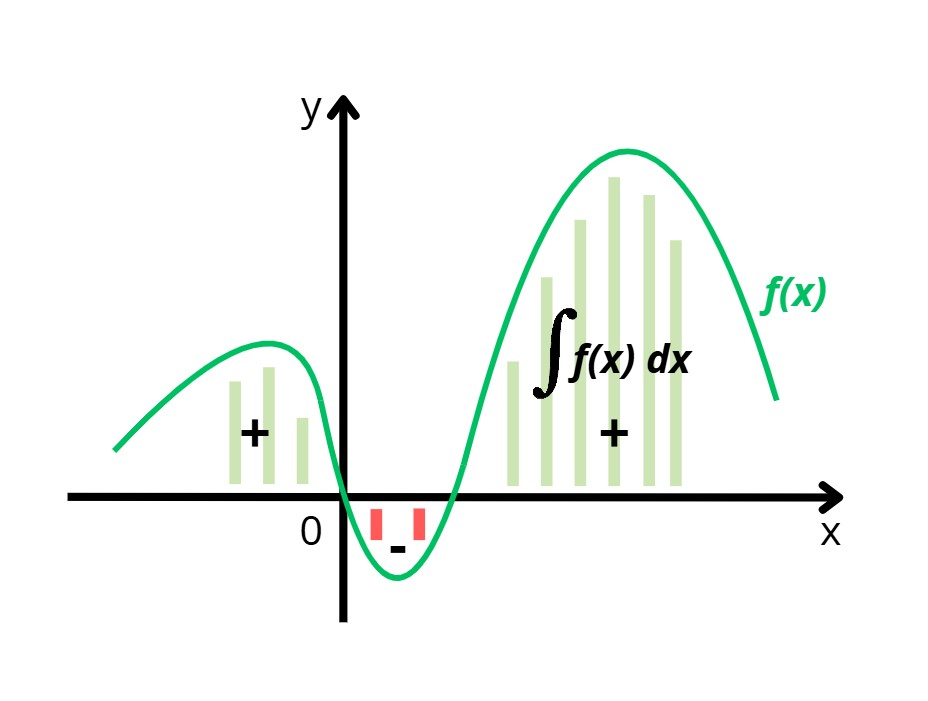
\includegraphics[width=0.6\textwidth]{images/cinematicGraphics/indefiniteIntegral.jpg}
    \caption*{Nota: Familia de funciones cuya derivada es la función dada.}
\end{figure}

\vspace{-40pt}

\[
\int f(x)\,dx = F(x) + C
\]

donde $F'(x) = f(x)$, es decir, $F(x)$ es una función cuya derivada es $f(x)$.

\textbf{Ejemplo:}
\[
\int 2x \, dx = x^2 + C
\]

porque:
\[
\frac{d}{dx}(x^2) = 2x
\]


\subsubsection{Integral definida}

\begin{figure}[H]
    \centering
    \captionsetup{width=0.5\textwidth}
    \caption{Interpretación gráfica de la integral definida}
    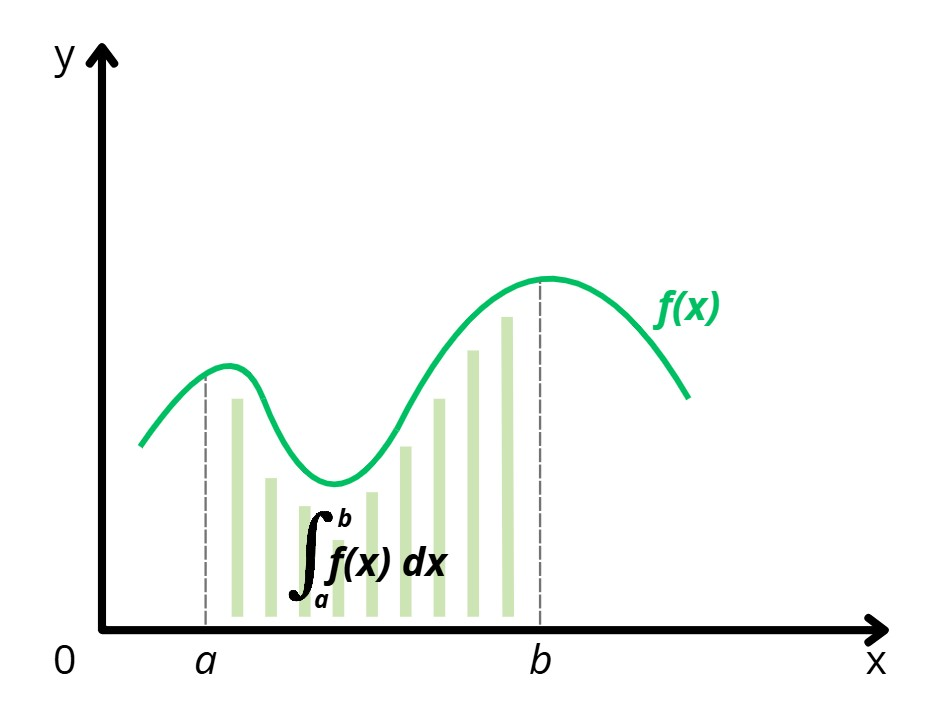
\includegraphics[width=0.6\textwidth]{images/cinematicGraphics/definiteIntegral.jpg}
    \caption*{Nota: Área bajo la curva en un intervalo determinado.}
\end{figure}

\vspace{-40pt}

\[
\int_a^b f(x)\,dx
\]

representa el área bajo la curva entre $a$ y $b$.

\textbf{Ejemplo:}
\[
\int_0^2 x \, dx
\]

Primero encontramos una primitiva:
\[
\int x \, dx = \frac{x^2}{2}
\]

Luego evaluamos en los límites:
\[
\left[\frac{x^2}{2}\right]_0^2 = \frac{2^2}{2} - \frac{0^2}{2}
\]
\[
= \frac{4}{2} - 0 = 2
\]

\subsubsection{Reglas de integración}

\begin{itemize}

\item \textbf{Regla de la potencia:}
\[
\int x^n dx = \frac{x^{n+1}}{n+1} + C
\]

\[
\int x^2 dx = \frac{x^3}{3} + C
\]

\item \textbf{Integral del coseno:}
\[
\int \cos x \, dx = \sin x + C
\]

\item \textbf{Integral del seno:}
\[
\int \sin x \, dx = -\cos x + C
\]

\end{itemize}
